\documentclass{beamer}

\usepackage[utf8]{inputenc}
\usepackage{graphicx}
\usepackage[autostyle]{csquotes}


\usefonttheme{serif}
\setbeamertemplate{navigation symbols}{}
\setbeamertemplate{footline}[frame number]{}

\hypersetup{
  colorlinks=true,
  linkcolor=blue
}

\newcommand{\vfbtitle}[1]{\begin{center}\Huge{#1}\end{center}}


\begin{document}

\begin{frame}[plain]
  \vfbtitle{Literate Programming}
\end{frame}

\begin{frame}
  \blockquote
  [\href{http://www.literateprogramming.com/knuthweb.pdf}{Literate Programming},
  Donald E. Knuth]{
    Let us change our traditional attitude to the construction of
    programs: Instead of imagining that our main task is to instruct a
    \textit{computer} what to do, let us concentrate rather on
    explaining to \textit{human beings} what we want a computer to do.
  }
\end{frame}

\begin{frame}
  \vfbtitle{Key points}

  \begin{itemize}
    \item Two artifacts: documentation and program
    \item Mostly prose, fragments of code
    \item Compiler-independent ordering
    \item Mostly a philosophical shift
  \end{itemize}
\end{frame}

\begin{frame}
  \begin{center}
    \includegraphics[scale=0.6]{flow.pdf}
  \end{center}
\end{frame}

\begin{frame}
  \vfbtitle{Demo}
\end{frame}

\begin{frame}
  \centering
  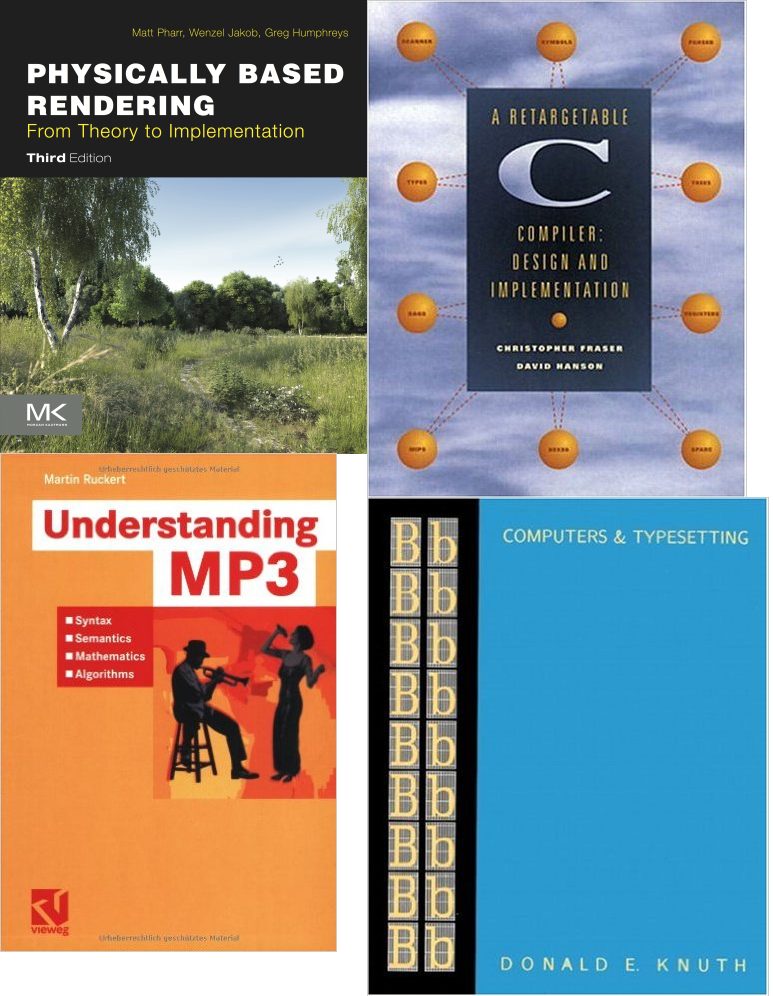
\includegraphics[scale=0.23]{media/lp-books.png}
\end{frame}

\begin{frame}
  \vfbtitle{The Bad}

  \begin{itemize}
    \item difficulty(LP) $>$ difficulty(code) $+$ difficulty(doc)
    \item Poor tool support
    \item Nobody does it
  \end{itemize}
\end{frame}


\begin{frame}
  \vfbtitle{The Good}

  \begin{itemize}
    \item Clear path to read (and understand) code
    \item Compiler-agnostic way to organize code
    \item Richer medium than ASCII
    \item Great aid 6 months from now
    \item ``Ce que l'on conçoit bien s'énonce clairement, Et les mots
    pour le dire arrivent aisément.'' (Nicolas Boileau)
  \end{itemize}
\end{frame}


\begin{frame}
  \vfbtitle{Discussion}

  \begin{itemize}
    \item Chunks as an extra means of abstraction
    \item How cohesive can a text written by tens of authors be?
    \item Where do unit tests go?
    \item Large programs?  Large refactorings?
  \end{itemize}
\end{frame}


\end{document}
